%
% File acl2019.tex
%
%% Based on the style files for ACL 2018, NAACL 2018/19, which were
%% Based on the style files for ACL-2015, with some improvements
%%  taken from the NAACL-2016 style
%% Based on the style files for ACL-2014, which were, in turn,
%% based on ACL-2013, ACL-2012, ACL-2011, ACL-2010, ACL-IJCNLP-2009,
%% EACL-2009, IJCNLP-2008...
%% Based on the style files for EACL 2006 by 
%%e.agirre@ehu.es or Sergi.Balari@uab.es
%% and that of ACL 08 by Joakim Nivre and Noah Smith

\documentclass[11pt,a4paper]{article}
\usepackage[hyperref]{acl2019}
\usepackage{times}
\usepackage{latexsym}
\usepackage{amssymb}
\usepackage{mathtools}
\usepackage{bussproofs}
\usepackage{libertine}
\usepackage{amsthm}
\usepackage{lineno}
\usepackage{url}
\usepackage{tikz}
%\usepackage{covington}

\newtheorem{theo}{Theorem}[section]  
\newtheorem{coro}[theo]{Corollary}

\theoremstyle{definition}
\newtheorem{defi}[theo]{Definition}

\newtheorem{thm}{Theorem}[section]
\newtheorem{defn}[thm]{Definition}
\newtheorem{lemma}[thm]{Lemma}
\newtheorem{prop}[thm]{Proposition}
\newtheorem{remark}[thm]{Remark}
\newtheorem{note}{Note}
\newtheorem{cor}[thm]{Corollary}
\newtheorem{example}[thm]{Example}


\aclfinalcopy % Uncomment this line for the final submission
%\def\aclpaperid{***} %  Enter the acl Paper ID here

%\setlength\titlebox{5cm}
% You can expand the titlebox if you need extra space
% to show all the authors. Please do not make the titlebox
% smaller than 5cm (the original size); we will check this
% in the camera-ready version and ask you to change it back.



\title{Exploring Lattice-based Models of Relevance in Dialogue for Questions and Implicatures}

\author{Julian Hough$^{1}$ and Andrew Lewis-Smith$^{2}$ \\
  $^{1}$Cognitive Science Group, $^{2}$Theory Group\\
  School of Electronic Engineering and Computer Science \\
  Queen Mary University of London\\
   \texttt{\{j.hough,a.lewis-smith\}@qmul.ac.uk}}


  
\date{}


\begin{document}
\sloppy
\maketitle
\begin{abstract}
We present work in-progress  on modelling relevance in dialogue for questions and implicatures, setting out a formal programme of work on reducing the redundancy which classical logic introduces into proofs. To do this we firstly propose the use of relevance logics, then set out a lattice-theoretic generalisation of Knuth's and Hough and Purver's models of questions and answers to achieve Belnap's First-degree Entailment.
\end{abstract}

%\section{Introduction}

%This document has been adapted from the instructions
%for earlier ACL and NAACL proceedings,
%including 
%those for 
%NAACL 2019 by Stephanie Lukin and Alla Roskovskaya, 
%ACL 2018 by Shay Cohen, Kevin Gimpel, and Wei Lu, 
%NAACL 2018 by Margaret Michell and Stephanie Lukin,
%2017/2018 (NA)ACL bibtex suggestions from Jason Eisner,
%ACL 2017 by Dan Gildea and Min-Yen Kan, 
%NAACL 2017 by Margaret Mitchell, 
%ACL 2012 by Maggie Li and Michael White, 
%those from ACL 2010 by Jing-Shing Chang and Philipp Koehn, 
%those for ACL 2008 by JohannaD. Moore, Simone Teufel, James Allan, and %Sadaoki Furui, 
%those for ACL 2005 by Hwee Tou Ng and Kemal Oflazer, 
%those for ACL 2002 by Eugene Charniak and Dekang Lin, 
%and earlier ACL and EACL formats.
%Those versions were written by several
%people, including John Chen, Henry S. Thompson and Donald
%Walker. Additional elements were taken from the formatting
%instructions of the \emph{International Joint Conference on Artificial
%  Intelligence} and the \emph{Conference on Computer Vision and
%  Pattern Recognition}.

\section{Introduction}
Formalizing what a relevant contribution consists of in a dialogue and particularly what constitutes a relevant answer to a question is now a classical problem for formal dialogue modelling. It has enjoyed a range of existing major treatments, clearly defined as a formal challenge from \newcite{Grice1975} onwards and made into a sub-discipline of pragmatics with Relevance Theory \cite{SperberWilson1986}.

Relevance was born out of Grice's original theory of \textit{implicature}, where speakers implicate hidden meaning which hearers can make sense of as in (\ref{eg:griceparty}) from \cite{Davis2014implicature}.

\vspace*{-0.35cm}
\begin{equation}
\label{eg:griceparty}
\text{
\begin{tabular}{ll}
    Alan: & Are you going to Paul's party?\\
    Barb: & I have to work.
\end{tabular}
}
\end{equation}
\vspace*{-0.35cm}

While a literal interpretation of Barb's contribution would not permit it to be judged a relevant answer to Alan's question, the unspoken meaning that she cannot attend is recoverable. Deriving from Grice's account, as \newcite{Davis2014implicature} notes, ``Neo-Gricean theories have modified Grice's principles to some extent, and Relevance theories replace them with a principle of communicative efficiency. The problems for such principle-based theories include overgeneration, lack of determinacy, clashes, and the fact that speakers often have other goals." We add to this criticism the failure to give \textit{real-valued} relevance measures to contributions, especially for answers to questions, though see \cite{HoughPurver2017Lattices} for one such approach in progress. In the current models the short polar answers `yes' and `no' would have the same degree of relevance as Barb's actual answer above, which is unintuitive.


\section{Implicature with relevance logic}

Here we explore some formal models of relevance agnostic to a theory of intention recognition, but which maintain the principle of least effort and maximising relevance in communication. To do this we look beyond classical logical approaches and move to a \textit{relevance logic} approach. We furthermore explore how real-valued relevance measures of answers to questions could be incorporated into such a framework through lattice theory. We are aiming for a model which would put a real value on the degree of relevance of the contribution if certain reasoning is applied to yield the unsaid meaning and implicature.



\begin{figure*}[!t]
    \centering
    \begin{tabular}{ll}
         1. & Barb can go to a party at time $T$ $\lor \neg$ Barb can go to a party at time $T$ $_{\{1\}}$ - \textit{question} \\
         2. & Barb is working at time $T$ $_{\{2\}}$ - \textit{statement} \\
         \hline
         3. & $\neg$ Barb can go to a party at time $T$ $_{\{2\}}$ - \textit{instantiation of work-party exclusion rule applied to 2} \\

        4. & ResolveQuestion(1,3) $_{\{1,2\}}$ - \textit{question resolution of question 1 by statement 3}
         
    \end{tabular}
    \caption{Deriving an implicated answer to a question by Relevance Logic proof.}
    \label{fig-relevancelogic}
\end{figure*}





Relevance in relevance logics is understood as ensuring every premise in a derivation is used in a proof. This has a connection in theoretical computer science to relevant type systems \cite{walker2005substructural} and numerous engineering applications,e.g. \cite{cheng2004temporal} or \cite{Bruns:2011:ACV:1952982.1952991}. %We illustrate this below. 
%\par Relevance logics, viewed independent of their algebraic semantics, have a special logical and proof-theoretic significance: they are $\it{substructural}$ $\it{logics}$, in that they result from viewing propositions and their proofs in a system as resources. Indeed, the Relevance logic $R$ arises from classical sequent calculus by removing the weakening rule \cite{paoli2013substructural} in analogous way to Linear Logic being the result of removing contraction and weakening from the classical Gentzen sequent system. 

In our example (\ref{eg:griceparty}) we assume Alan and Barb would both have access to a general reasoning rule that may be available as a resource or reasoning pattern like (\ref{def:workpartyexclusion}).

\vspace*{-0.5cm}
\begin{align}
    \label{def:workpartyexclusion}  \text{X is working at time }T \rightarrow \nonumber \\
    \neg\text{ X can go to a party at time }T\nonumber \\
    \textit{(work-party exclusion rule)}
\end{align}
\vspace*{-0.5cm}

This rule tells us when someone is working they cannot attend a party (fairly reasonable consideration for most, unless one works in e.g catering, clown acts, etc.). With this rule to hand, in the spirit of \cite{Breitholtz2014}, we can derive a proof of the implicature that Barb cannot go to the party at that time which can resolve Alan's question, as shown in Fig.~\ref{fig-relevancelogic}. We use \newcite{Mares2004}'s logical notation where the curly brackets containing the indices of the premises used in that line. The proof in Fig.~\ref{fig-relevancelogic} shows how both premises are used to derive the conclusion in line 4, which itself uses the implicature in line 3.

While this seems better than a classical logic approach because redundancy is minimized, the problem remains that we still don't have a handle on a real-valued relevance which could lead to a computational model of selecting relevant rules.

\section{Towards Relevance Logic Lattices for Real-valued Relevance}





To model the real-valued relevance of answers to questions and implicatures, we look to work by \newcite{knuth2005lattice} and \cite{HoughPurver2017Lattices} whereby a boolean algebra statement lattice like that in Fig.~\ref{fig:knuthlattice} in the Appendix allows real-valued probabilities to be assigned to the atoms of the lattice and then consequently to the joins of those elements. Questions are derived from this lattice as the joins of all the downsets of these elements. In such a framework in our example in Fig.~\ref{fig-relevancelogic}, a relevance value is contingent on the the real-valued inclusion of statement 3 in statement 2 on the lattice after the application of the `work-party exclusion rule'-- if this is sufficiently high, we could rule this a relevant application of the general rule in order to derive 4. 

While this seems to give us what we want, a problem of relevance remains, but this time in terms of the available answers to questions: in Knuth's analysis, all questions can trivially evaluate to $\bot$. In fact $\top$ in Knuth's analysis is co-extensive with the entire space of questions and answers, which is counter-intuitive for any question with any content that does not involve asking whether something is true or false. We propose adopting a different underlying algebra which helps block these issues, and seems to capably model relevance both as a conversational implicature and as a logical consequence relation.  We believe this can be achieved through a De Morgan lattice like Fig.~\ref{fig:lattices} where the trivial results can be minimized and we can achieve a Relevant logic known as First-Degree Entailment (FDE). \cite{Belnap1977} and their collaborators \cite{anderson2017entailment} show how this can be achieved-- see Fig.~\ref{fig:fde} Appendix for an illustration.

\begin{figure}[!t]
\begin{center}

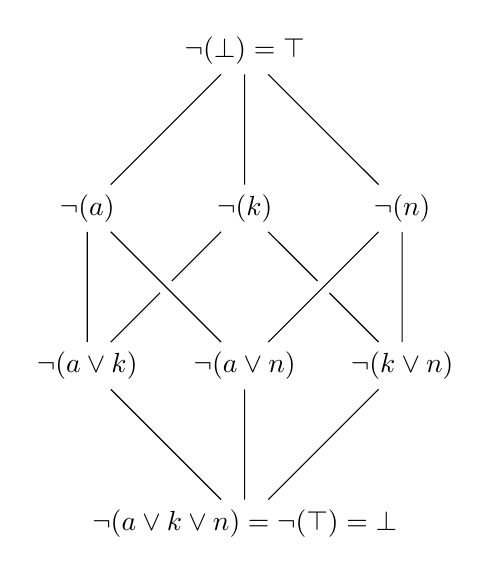
\begin{tikzpicture}
  \node (max) at (0,4) {$\neg(\bot) = \top$};
  \node (a) at (-2,2) {$\neg(a)$};
  \node (b) at (0,2) {$\neg(k)$};
  \node (c) at (2,2) {$\neg(n)$};
  \node (d) at (-2,0) {$\neg(a \lor k)$};
  \node (e) at (0,0) {$\neg(a \lor n)$};
  \node (f) at (2,0) {$\neg(k \lor n)$};
  \node (min) at (0,-2) {$\neg(a \lor k \lor n) = \neg(\top) = \bot$};
  \draw (min) -- (d) -- (a) -- (max) -- (b) -- (f)
  (e) -- (min) -- (f) -- (c) -- (max)
  (d) -- (b);
  \draw[preaction={draw=white, -,line width=6pt}] (a) -- (e) -- (c);
\end{tikzpicture}
\end{center}
\vspace*{-0.35cm}
\caption{De Morgan lattice}\label{fig:lattices}
\end{figure}

\section{Future Work}
In future work we would like to leverage the power of Knuth's work on probability and information theory with question and statement lattices and the De Morgan lattices described above for deriving a real-valued relevance of a contribution resolving the central issue. We have evidence that Knuth's approach can be generalised and De Morgan algebras are, in addition to being the backbone of FDE described above, investigated in fuzzy logic circles-- for example forming an adequate algebraic semantics for a Lukasiewicz logic \cite{Nguyen:1996:FCF:235242}. 



\iffalse
\section{Algebras for Questions}
\subsection{Knuth and Lattices}
Our starting point for a formal analysis of questions and relevance is Knuth's ~\cite{knuth2005lattice}, in which he employs Boolean lattices as a means for analysing questions and answers in dialogue. Defining $x \le y = x \rightarrow y$, he suggests that two questions are equivalent if they are answered by the
same set of assertions. \par In using his definition of implication as defined on a lattice ordering, he can exploit natural properties of the lattice to conclude what the answers to a given question should be. Take the following example from ~\cite{knuth2005lattice}. `Who stole the tarts made by the Queen of Hearts?' is the question. For his example, there are three mutually exclusive statements $a, k$ or $n$ for `Alice stole the tarts!', `The Knave of Hearts stole the tarts!'or `No one stole the tarts!' respectively. We are told only one of these answers his question. The assertion lattice is depicted below:

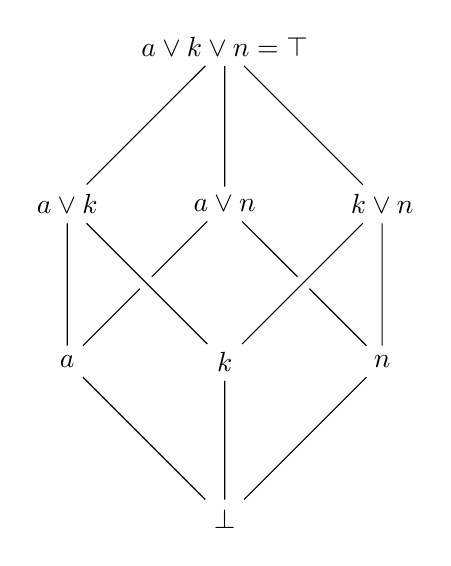
\begin{tikzpicture}
  \node (max) at (0,4) {$a \lor k \lor n = \top$};
  \node (a) at (-2,2) {$a \lor k$};
  \node (b) at (0,2) {$a \lor n$};
  \node (c) at (2,2) {$k \lor n$};
  \node (d) at (-2,0) {$a$};
  \node (e) at (0,0) {$k$};
  \node (f) at (2,0) {$n$};
  \node (min) at (0,-2) {$\bot$};
  \draw (min) -- (d) -- (a) -- (max) -- (b) -- (f)
  (e) -- (min) -- (f) -- (c) -- (max)
  (d) -- (b);
  \draw[preaction={draw=white, -,line width=6pt}] (a) -- (e) -- (c);
\end{tikzpicture}

In Knuth's analysis, if an assertion $x$ answers a question, then then the set of assertions $y$ that imply $x$ also answer that question. 

\defn[Downsets] Let $\mathfrak{L}$ be a lattice. Then for all $x,y \in \mathfrak{L}$, the $\it{Downset}$ formed from $x$: $\downarrow x = \{y | y \le x\}$ \\
Using the latter and the more general algebraic construction of $\it{order}$ $\it{ideals}$, Knuth can do two things exploiting the underlying Boolean algebra of assertions for a given question:
\begin{enumerate}
    \item Deduce the answers to a given question;
    \item Produce the lattice of questions for which the assertion lattice provides answers.
\end{enumerate}
\example \label{sec-example}If indeed Alice stole the tarts, $\downarrow$$a = \{\bot, a\}$ gives the answer set to the question of who stole the tarts (Alice and $\bot$).\\ 
\par This construction introduces irrelevance in the answer set: $\bot$ conveys no information at all ($\bot$ is not a person in the domain but a constant across Boolean algebras), yet by Knuth's construction $\bot$ is in $\it{every}$ answer set. This is undesirable, for intuitively, if we know one or more answers are correct and relevant for a question, we want those answers alone. This means we seek to rule out trivialities and vacuous information in our answer set. \footnote{Similarly, as $\bot = a \land \neg a$ in a Boolean algebra, $a \land \neg a$ is an odd answer to the question of who stole the tarts, but it is nonetheless valid under the present model, and will answer every question posed, as it is equivalent to $\bot$.} % \footnote{There are more issues of irrelevance here as well. For instance, since ideals ( all downsets are ideals) are closed under finite join, if $\{\bot, a\}$ is an ideal in the assertion lattice, and $a \lor a$ is an answer given by this ideal. This is irrelevant, as if $a$ really is true, even if $a \lor a$ is trivially true we would not want it in our answer set as it conveys no more information than $a$.} 
%~\ref{sec:length}.


\subsection{De Morgan Algebras}
With this in mind, we have two observations which we think can resolve the above problem. 
\begin{enumerate}
    \item Change the construction.
    \item Change the algebra.\footnote{Both are necessary, as improving the construction does not affect the global irrelevance of the underlying algebra (and doesn't guarantee us the connection to FDE). In changing the algebra one gains tighter control over the answer set, but the construction must still be modified slightly to preserve the desired relevant answers.}
\end{enumerate}

\defn[De Morgan Algebras] $\mathfrak{A} = (A, \lor, \land, \bot, \top)$ is a bounded distributive lattice, and
$\neg$ is a De Morgan involution: $\neg(x \land y) = \neg 
x \lor \neg y$ and $\neg\neg x = x$. We say that $\mathfrak{A}$ is a De Morgan Algebra.

\note $\mathfrak{A}$ is a proper subalgebra of the Boolean algebra, as $(x \land \neg x) \neq \bot$ and $(x \lor \neg x) \neq \top$. If we add $(x \land \neg x) = \bot$ or its dual, we obtain a Boolean algebra. 

\defn[Modified Downsets] Define $\downarrow x\prime := \downarrow x \setminus \{\bot\}$. In words: $\downarrow x\prime$ is the downset relation of before, but without $\bot$. 

\example cf. \ref{sec-example} : $\downarrow x\prime = \{a\}$.

\remark These considerations give us a tighter control over the set of relevant questions. To see that this is so in the setting of Knuth's example, take the assertion lattice. Since $\neg$ is a dual automorphism on the algebra, we get the following by inverting the lattice:

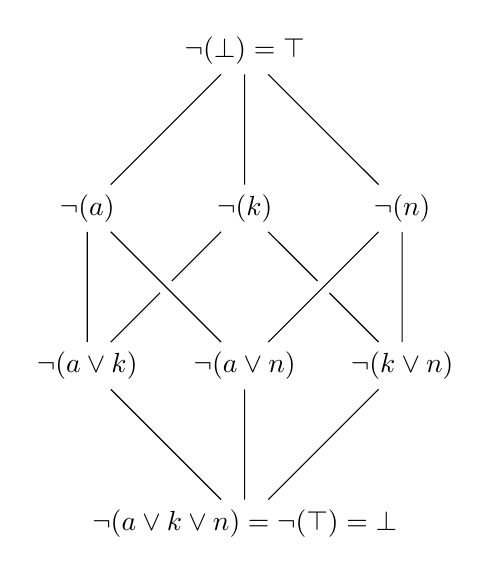
\begin{tikzpicture}
  \node (max) at (0,4) {$\neg(\bot) = \top$};
  \node (a) at (-2,2) {$\neg(a)$};
  \node (b) at (0,2) {$\neg(k)$};
  \node (c) at (2,2) {$\neg(n)$};
  \node (d) at (-2,0) {$\neg(a \lor k)$};
  \node (e) at (0,0) {$\neg(a \lor n)$};
  \node (f) at (2,0) {$\neg(k \lor n)$};
  \node (min) at (0,-2) {$\neg(a \lor k \lor n) = \neg(\top) = \bot$};
  \draw (min) -- (d) -- (a) -- (max) -- (b) -- (f)
  (e) -- (min) -- (f) -- (c) -- (max)
  (d) -- (b);
  \draw[preaction={draw=white, -,line width=6pt}] (a) -- (e) -- (c);
\end{tikzpicture}

In particular, $a \land \neg a \neq \bot$.%\footnote{The use of $\prime$ merely indicates that the resultant $\top$ or $\bot$ results from an involution of the old $\top$ and $\bot$.}
\remark Note that $\top$ and $\bot$ still hold their rightful places in the ordering and the behavior of the lattice is otherwise familiar. This structure is just weak enough to carry out much of Knuth's analysis but strong enough to sieve out irrelevant assertions. It turns out this connection is more than skin deep.
\section{Relevance via Logic}
\subsection{The Connection with Relevance logics}
De Morgan algebras have been studied at least since \cite{10.2307/1993112} as algebras in their own right, but work of Dunn \cite{Dunn1999}, Belnap \cite{Belnap1977} and their collaborators \cite{anderson2017entailment} conveys a deep connection between De Morgan algebras and a Relevant logic known to cognoscenti as First-Degree Entailment (FDE). The logic itself is one of the first successfully explored variants of Relevant logic, and indeed has a variety of semantics on offer (relational, matrices, algebraic), each of which are formally adequate for the system \cite{omori201740}. The key is that the algebraic semantics delivers insights not easily derived by matrix calculations or relational semantics, and forms the most general semantic perspective on offer for FDE, and serves as a blueprint for further generalisation in other cases (De Morgan Monoids, Dunn monoids, etc.). 
\subsection{Belnap's FDE}
\par Sadly, there is not one best system of relevance logic - there are many varieties of relevance logics \cite{anderson2017entailment}. \ref{table-fde-logic} presents a sequent-style natural deduction system for FDE (also found in \cite{omori201740}).
\fi





%\newpage
\begingroup
\sloppy

\bibliographystyle{acl_natbib}
\bibliography{refs} 
\endgroup
\appendix


\newpage
\section*{Appendix}
\label{sec:appendix}


\begin{figure}[!h]
\begin{center}
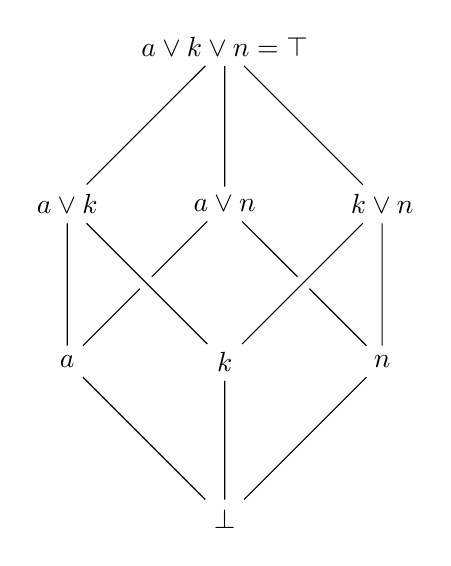
\begin{tikzpicture}
  \node (max) at (0,4) {$a \lor k \lor n = \top$};
  \node (a) at (-2,2) {$a \lor k$};
  \node (b) at (0,2) {$a \lor n$};
  \node (c) at (2,2) {$k \lor n$};
  \node (d) at (-2,0) {$a$};
  \node (e) at (0,0) {$k$};
  \node (f) at (2,0) {$n$};
  \node (min) at (0,-2) {$\bot$};
  \draw (min) -- (d) -- (a) -- (max) -- (b) -- (f)
  (e) -- (min) -- (f) -- (c) -- (max)
  (d) -- (b);
  \draw[preaction={draw=white, -,line width=6pt}] (a) -- (e) -- (c);
\end{tikzpicture}

\end{center}
\caption{A Knuth-style lattice of statements for a Boolean algebra}\label{fig:knuthlattice}
\end{figure}


\begin{figure}[!h]
\begin{minipage}{.35\textwidth}
    %    
    \begin{prooftree}
    \AxiomC{$\Gamma \vdash \phi$}
    \AxiomC{$\Gamma \vdash \psi$}
    \RightLabel{\scriptsize{$\land$ I}}
    \BinaryInfC{$\Gamma \vdash \phi \land \psi$}
    \end{prooftree}
    %
    \begin{prooftree}
    \AxiomC{$\Gamma \vdash \phi_i$}
    \RightLabel{\scriptsize{$\lor$ I \; $(i \in \{1,2\})$}}
    \UnaryInfC{$\Gamma \vdash \phi_1 \lor \phi_2$}
    \end{prooftree}
    %
    \end{minipage}
    \begin{minipage}{.55\textwidth}
    %
    %
    \begin{prooftree}
    \AxiomC{$\Gamma \vdash \phi_1 \land \phi_2$}
    \RightLabel{\scriptsize{$\land$ E \; $(i \in \{1, 2\})$}}
    \UnaryInfC{$\Gamma \vdash \phi_i$}
    \end{prooftree}
    %
    \begin{prooftree}
    \AxiomC{$\Gamma \vdash \phi \lor \psi$}
    \AxiomC{$\Delta, \phi \vdash \chi$}
    \AxiomC{$\Delta, \psi \vdash \chi$}
    \RightLabel{\scriptsize{$\lor$ E}}
    \TrinaryInfC{$\Gamma, \Delta \vdash \chi$}
    \end{prooftree}
    %
    \begin{prooftree}
    \AxiomC{$\Gamma \vdash \neg\neg\phi$}
    \RightLabel{\scriptsize{$\neg$$\neg$ E \;}}
    \UnaryInfC{$\Gamma \vdash \phi$}
    \end{prooftree}
    %
    \begin{prooftree}
    \AxiomC{$\Gamma \vdash \phi$}
    \RightLabel{\scriptsize{$\neg$$\neg$ I \;}}
    \UnaryInfC{$\Gamma \vdash \neg\neg\phi$}
    \end{prooftree}
    %
    \begin{prooftree}
    \AxiomC{$\Gamma \vdash \neg(\phi \lor \psi)$}
    \RightLabel{\scriptsize{DeMorgan(i) \;}}
    \UnaryInfC{$\Gamma \vdash \neg\phi \land \neg\psi$}
    \end{prooftree}
    %
    \begin{prooftree}
    \AxiomC{$\Gamma \vdash \neg(\phi \land \psi)$}
    \RightLabel{\scriptsize{DeMorgan(ii) \;}}
    \UnaryInfC{$\Gamma \vdash \neg\phi \lor \neg\psi$}
    \end{prooftree}
    %
\end{minipage} 
\caption{FDE}
\label{fig:fde}
\end{figure}





%where \verb|acl2019| corresponds to a acl2019.bib file.


%\appendix

%\section{Appendices}
%\label{sec:appendix}
%Appendices are material that can be read, and include lemmas, formulas, proofs, and tables that are not critical to the reading and understanding of the paper. 
%Appendices should be \textbf{uploaded as supplementary material} when submitting the paper for review. Upon acceptance, the appendices come after the references, as shown here. Use
%\verb|\appendix| before any appendix section to switch the section
%numbering over to letters.


%\section{Supplemental Material}
%\label{sec:supplemental}
%Submissions may include non-readable supplementary material used in the work and described in the paper. Any accompanying software and/or data should include licenses and documentation of research review as appropriate. Supplementary material may report preprocessing decisions, model parameters, and other details necessary for the replication of the experiments reported in the paper. Seemingly small preprocessing decisions can sometimes make a large difference in performance, so it is crucial to record such decisions to precisely characterize state-of-the-art methods. 

%Nonetheless, supplementary material should be supplementary (rather
%than central) to the paper. \textbf{Submissions that misuse the supplementary 
%material may be rejected without review.}
%Supplementary material may include explanations or details
%of proofs or derivations that do not fit into the paper, lists of
%features or feature templates, sample inputs and outputs for a system,
%pseudo-code or source code, and data. (Source code and data should
%be separate uploads, rather than part of the paper).

%The paper should not rely on the supplementary material: while the paper
%may refer to and cite the supplementary material and the supplementary %material will be available to the
%reviewers, they will not be asked to review the
%supplementary material.


\end{document}
